% CORA.cpp and CORALean: backends, bindings, and the equivalence of their results
\documentclass[tikz,border=6pt]{standalone}
\usetikzlibrary{arrows.meta,positioning,calc}

\definecolor{CORAcolorBlue}{rgb}{0, 0.4470, 0.7410}
\definecolor{CORAcolorRed}{rgb}{0.8500, 0.3250, 0.0980}
\definecolor{CORAcolorGreen}{rgb}{0.4660, 0.6740, 0.1880}

\begin{document}
\sffamily
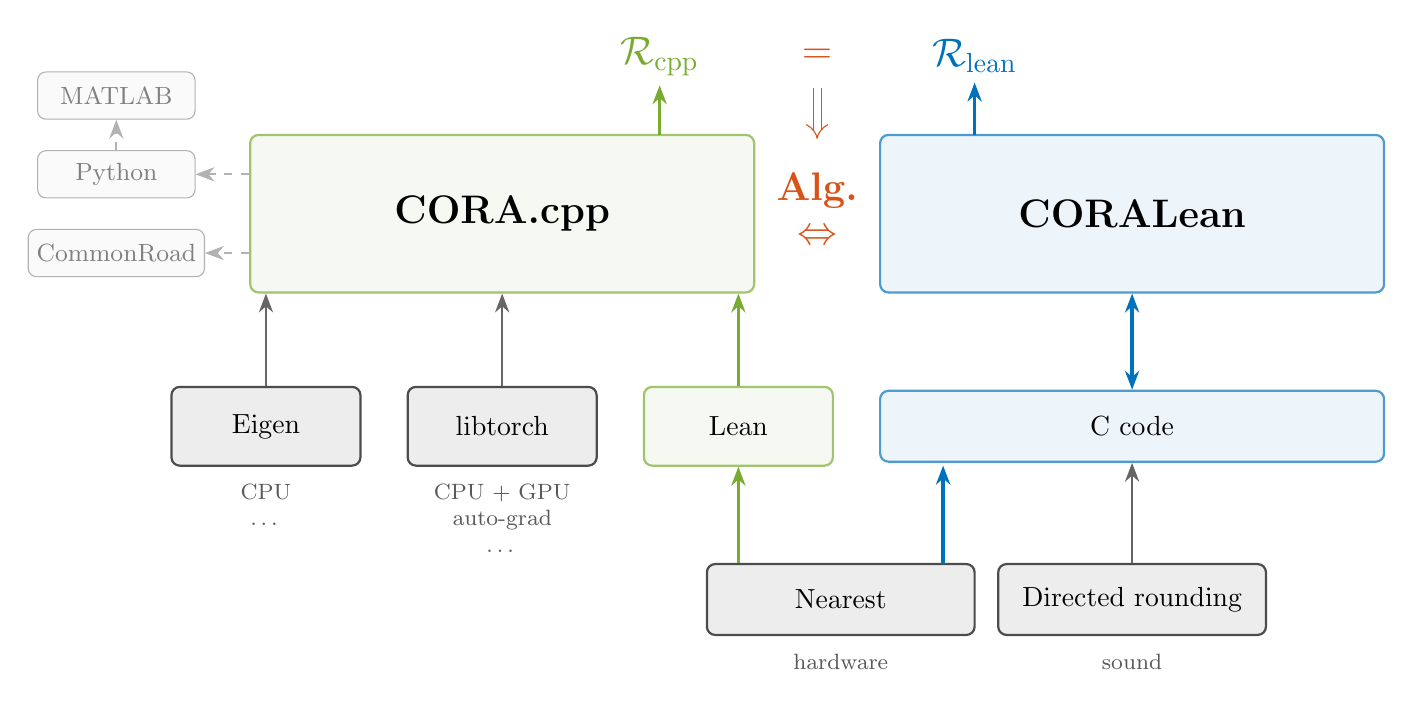
\begin{tikzpicture}[
    >={Stealth[length=2.4mm]},
    box/.style={draw=#1!70, fill=#1!7, rounded corners=3pt, thick, align=center,
                minimum height=9mm, inner sep=4pt},
    box/.default=black,
    big/.style={box=#1, minimum width=64mm, minimum height=20mm, font=\Large\bfseries},
    sub/.style={box=#1, minimum width=24mm, minimum height=10mm},
    bind/.style={draw=black!30, fill=black!2, rounded corners=3pt, align=center,
                 minimum height=6mm, minimum width=20mm, inner sep=3pt, text=black!50,
                 font=\small},
    note/.style={font=\footnotesize, text=black!65, align=center, text width=26mm},
    link/.style={thick, ->, draw=black!60},
    faint/.style={->, draw=black!30, thick, dashed},
    cpp/.style={very thick, ->, draw=CORAcolorGreen},
    lean/.style={very thick, ->, draw=CORAcolorBlue},
    res/.style={font=\Large, text=CORAcolorRed},
]

% toolboxes, mirrored about x = 4
\node[big=CORAcolorGreen] (cpp) at (0,0) {CORA.cpp};
\node[big=CORAcolorBlue] (lean) at (8,0) {CORALean};

% bindings, off to the side
\node[bind] (matlab) at (-4.9,1.5) {MATLAB};
\node[bind] (python) at (-4.9,0.5) {Python};
\node[bind] (commonroad) at (-4.9,-0.5) {CommonRoad};
\draw[faint] (cpp.west |- python) -- (python.east);
\draw[faint] (cpp.west |- commonroad) -- (commonroad.east);
\draw[faint] (python.north) -- (matlab.south);

% CORA.cpp backends
\node[sub=black] (eigen) at (-3,-2.7) {Eigen};
\node[sub=black] (torch) at (0,-2.7) {libtorch};
\node[sub=CORAcolorGreen] (leanb) at (3,-2.7) {Lean};
\node[note, below=1mm of eigen] {CPU \\ \dots};
\node[note, below=1mm of torch] {CPU + GPU \\ auto-grad \\ \dots};
\foreach \b in {eigen, torch}
    \draw[link] (\b.north) -- (\b.north |- cpp.south);
\draw[cpp] (leanb.north) -- (leanb.north |- cpp.south);

% CORALean side
\node[box=CORAcolorBlue, minimum width=64mm] (ccode) at (8,-2.7) {C code};
\draw[lean, <->] (lean) -- (ccode);

% rounding modes
\node[box=black, minimum width=34mm] (nearest) at (4.3,-4.9) {Nearest};
\node[note, below=1mm of nearest] {hardware};
\node[box=black, minimum width=34mm] (directed) at (8,-4.9) {Directed rounding};
\node[note, below=1mm of directed] {sound};
\draw[cpp] (leanb.south |- nearest.north) -- (leanb.south);
\draw[lean] (5.6,-4.45) -- (5.6,-3.2);
\draw[link] (directed.north) -- (directed.north |- ccode.south);

% results, mirrored about x = 4
\node[res] (eq) at (4,2.0) {$=$};
\node[res, text=CORAcolorGreen] (rcpp) at (2,2.0) {$\mathcal{R}_{\mathrm{cpp}}$};
\node[res, text=CORAcolorBlue] (rlean) at (6,2.0) {$\mathcal{R}_{\mathrm{lean}}$};
\draw[cpp] (2,1.0) -- (rcpp.south);
\draw[lean] (6,1.0) -- (rlean.south);
\draw[-{Implies[length=4mm]}, double distance=2.5pt, draw=CORAcolorRed] (4,1.6) -- (4,0.95);
\node[res, font=\Large\bfseries] (algo) at (4,0.3) {Alg.};
\node[res] at (4,-0.3) {$\Leftrightarrow$};
\end{tikzpicture}
\end{document}
